\documentclass{beamer}
\usetheme{metropolis}
\usepackage{graphicx}
\usepackage{subfig}
\usepackage{hyperref}
\usepackage{tcolorbox}
\title{Calculus-Based Physics-1: Mechanics (PHYS150-02): Unit 6}
\date{\today}
\author{Jordan Hanson}
\institute{Whittier College Department of Physics and Astronomy}

\begin{document}
\maketitle

\section{Unit 6 Summary}

\begin{frame}{Week 6 Summary}
\begin{enumerate}
\item \alert{Work} has a scientifically precise definition
\begin{itemize}
\item Units
\item As a product of force and displacement vectors
\end{itemize}
\item Kinetic Energy and the \alert{Work-Energy Theorem}
\item Gravitational potential energy
\begin{itemize}
\item Potential energy
\item \textit{Simplifying otherwise complex calculations}
\item Potential energy near Earth's surface
\item ...in space
\end{itemize}
\item Definition of a \textbf{conservative force}
\begin{itemize}
\item Relationship between conservative forces and potential energy
\item Conservation of energy for conservative forces
\end{itemize}
\end{enumerate}
\end{frame}

\section{Definitions of Work}

\begin{frame}{Definitions of Work}
\begin{tcolorbox}[colback=white,colframe=red!40!blue,title=Physical Definition of Work]
\alert{Let $\vec{F}$ be a force exerted on a system, which is displaced by a displacement $\vec{x}$.  The \textbf{work} done on the system is} \\
\alert{$W = \vec{F} \cdot \vec{x}$} \\
\end{tcolorbox}
The units of work are N m = kg m/s$^2$, or \textit{Joules}. \\
\vspace{0.5cm}
\small
\textit{Extra credit opportunity}: \textbf{Do you like beer}?  Write a 10-page paper on the on the scientific challenge faced by James Prescott Joule, who began to formulate the modern view of energy in the 19th century, contrary to \textit{caloric theory}.  \textbf{Upon completion of this assignment I will change two homework scores to perfect scores.}
\end{frame}

\begin{frame}{Definitions of Work}
Let $\theta$ be the angle between the force and the displacement.  Then this equation
\begin{equation}
W = \vec{F} \cdot \vec{x}
\end{equation}
becomes
\begin{equation}
W = Fx\cos\theta
\end{equation}
\end{frame}

\begin{frame}{Definitions of Work}
\begin{figure}
\centering
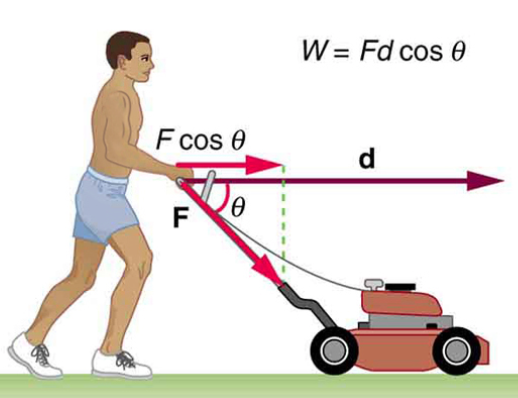
\includegraphics[width=0.7\textwidth]{figures/lawn.png}
\caption{\label{fig:work} A case where $\theta \neq 0$.}
\end{figure}
\end{frame}

\begin{frame}{Definitions of Work}
\begin{figure}
\centering
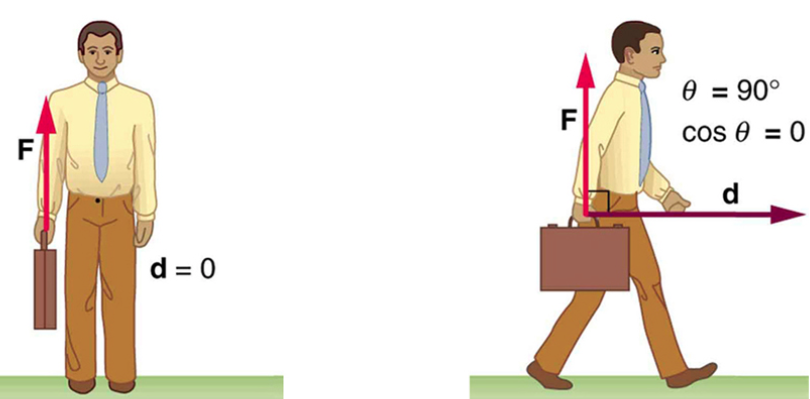
\includegraphics[width=0.7\textwidth]{figures/lawn2.png}
\caption{\label{fig:work2} (Left): A case where $x = 0$, so $W=0$.  (Right): A case where $\theta = 90^{\circ}$, so $W=0$.}
\end{figure}
\small
Just because an action requires \textit{energy} doesn't mean we are performing \textit{work}.  It requires muscular energy to hold up a heavy briefcase but this is not what we mean by work.  Work is about moving objects.
\end{frame}

\begin{frame}{Definitions of Work}
What about Newton's 3rd Law?  If one system $A$ exerts a force $F_{\rm AB}$ on a system $B$, then Newton's 3rd law states that system $B$ exerts a force $-F_{\rm AB}$ on system A. \\
\vspace{0.5cm}
If \alert{the work done by $A$ on $B$} is $W = (F_{\rm AB})x\cos\theta$, then \alert{the work done by $B$ on $A$} is $W = -(F_{\rm AB})x\cos\theta$. \\
\vspace{0.5cm}
In Fig. \ref{fig:work}, the work done by the man on the mower is positive, but the work done by the mower on the man is negative.
\end{frame}

\begin{frame}{Definitions of Work}
\small
More units of energy:
\begin{table}
\centering
\begin{tabular}{c | c | c}
\alert{Unit Name} & \alert{Definition} & \alert{Value} \\ \hline
electron-volt (eV) & energy of 1 e$^{-}$ through 1 V & $1.60\times 10^{-19}$ J \\ \hline
1 Rydberg (Rd) & ionize 1 hydrogen atom & $21.8\times 10^{-19}$ J \\ \hline
\textbf{Joule} & \textbf{1 N$\cdot$m} & \textbf{1.0 J} \\ \hline
foot-pound & 1 ft$\cdot$lb & 1.36 J \\ \hline 
calorie & Raise 1 gram of water 1$^{\circ}$ C & 4.184 J \\ \hline
British Thermal Unit & Raise 1 lb of ice to boil ($^{\circ}$F) & 1054.3 J \\ \hline
food calorie (kcal) & 1000 calories & 4184 J \\ \hline
kilowatt hours & 1 kilowatt system for 1 hr & $3.6\times 10^6$ J \\ \hline
gasoline galon equiv. & burning a galon of gas & $\approx 120 \times 10^6$ J \\ \hline
$E = mc^2$, 1 mole of H$^{+}$ & Rest mass (fusion/fission) & $9 \times 10^{13}$ J \\ \hline
\end{tabular}
\end{table}
\end{frame}

\begin{frame}{Definitions of Work}
\begin{figure}
\centering
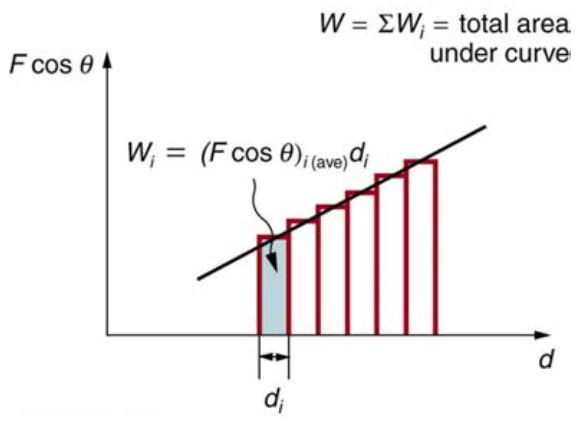
\includegraphics[width=0.6\textwidth]{figures/integral.png}
\caption{\label{fig:work3} Breaking the displacement $\vec{x}$ into pieces, and summing them.}
\end{figure}
\small
This interpretation naturally leads to the subject of \textit{integration} in calculus.  
\end{frame}

\begin{frame}{Definitions of Work}
\begin{figure}
\centering
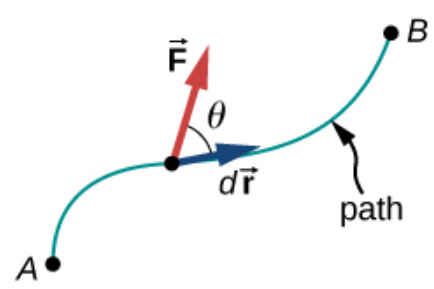
\includegraphics[width=0.4\textwidth]{figures/line.png}
\caption{\label{fig:line} Summary of the concept of the work integral.}
\end{figure}
\begin{equation}
W = \int_{AB} \vec{F} \cdot d\vec{r}
\end{equation}
\end{frame}

\begin{frame}{Definitions of Work}
Consider the case where the force doing the work on the system of mass $m$ is friction:
\begin{equation}
W = \int_{AB} \vec{F} \cdot d\vec{r} = -\int_{AB} \mu_{\rm k} N dx = -\mu_{\rm k} m g \int_{AB} dx 
\end{equation}
\small
\begin{itemize}
\item Friction acts in opposite direction, so the dot product gives a minus sign
\item Friction acts along path $AB$ (whatever direction of motion is)
\end{itemize}
\end{frame}

\begin{frame}{Definitions of Work}
The driver of a 900 kg car slams on the breaks, and the tires slide on the pavement with $\mu_{\rm k} = 0.2$.  The initial speed is 25 m/s.  Assuming $g = 10$ m/s$^2$, how far does the car travel before coming to a stop?
\begin{itemize}
\item A: 312.5 m
\item B: 625 m
\item C: 31.25 m
\item D: 62.5 m
\end{itemize}
\end{frame}

\begin{frame}{Definitions of Work}
What is the work done on the car?
\begin{itemize}
\item A: 280 J
\item B: -280 J
\item C: 280 kJ
\item D: -280 kJ
\end{itemize}
\end{frame}

\begin{frame}{Definitions of Work}
Take your \textit{algebraic} answer for the breaking distance (displacement from two slides ago), and substitute it into the expression for the work done on the car (force of friction times displacement).  What do you get?  (\textit{Check your units}).
\begin{itemize}
\item A: $m v_{\rm i}^2$
\item B: $m g \frac{1}{2} m v_{\rm i}^2$
\item C: $-\frac{1}{2} m v_{\rm i}^2$
\item D: $\mu_{\rm k} m v_{\rm i}^2$
\end{itemize}
\textit{Keep this result in mind}...
\end{frame}

\begin{frame}{Definitions of Work}
Suppose we raise the 900 kg car by a displacement of 10 meters.  What is the work done on the car?
\begin{itemize}
\item A: 9 J
\item B: 90 J
\item C: 900 kJ
\item D: 90 kJ
\end{itemize}
\end{frame}

\begin{frame}{Definitions of Work}
What if we drop the car from a height of 10 m?  What is the final velocity of the car?
\begin{itemize}
\item A: $10\sqrt{2}$ m/s
\item B: $20$ m/s
\item C: $10$ m/s
\item D: $10\sqrt{10}$ m/s
\end{itemize}
\end{frame}

\begin{frame}{Definitions of Work}
Stand up, and show in your groups that the work done on the falling car is equal to $\frac{1}{2}m v_{\rm f}^2$, both numerically and algebraically.
\end{frame}

\section{Applications of the Concept of Work}

\begin{frame}{Applications of the Concept of Work}
\textbf{Work done on an oscillator}.  Let $\vec{x}$ be the displacement of a mass $m$ attached to an oscillator (a spring), with spring constant $k$.  The spring applies a force $\vec{F}$ to the mass:
\begin{align}
F &= -kx \\
W &= \int \vec{F} \cdot d\vec{x} \\
W &= -k\int_{AB} x dx = -\frac{1}{2}k x^2 \label{eq:sp}
\end{align}
Equation \ref{eq:sp} the work done \textit{on the mass by the spring}.  The work performed \textit{by the system applying the force is}:
\begin{equation}
W_{\rm spring} = \frac{1}{2}k x^2
\end{equation}
\end{frame}

\begin{frame}{Applications of the Concept of Work}
Work done on an oscillator:
\begin{equation}
W_{\rm spring} = \frac{1}{2}k x^2
\end{equation}
\textit{For two points A and B that are neither at equilibrium point of oscillator}:
\begin{equation}
W_{\rm spring,AB} = \frac{1}{2}k x_{\rm B}^2 - \frac{1}{2}k x_{\rm A}^2 = \frac{1}{2}k(x_{\rm B}^2 - x_{\rm A}^2)
\end{equation}
\end{frame}

\begin{frame}{Applications of the Concept of Work}
What about gravity as the force?
\begin{equation}
W_{\rm g} = \int_{A}^{B} -mg \hat{j} \cdot dy \hat{j} = -mg(y_{\rm B} - y_{\rm A}) = -mg\Delta y
\end{equation}
\textit{Why the minus sign?}  Gravity does negative work if we raise an object $\Delta y$.  We contribute $W_{\rm g} = mg\Delta y$ (J) of energy to raise an object $\Delta y$ against gravity.
\end{frame}

\begin{frame}{Applications of the Concept of Work}
\begin{columns}[T]
\begin{column}{0.5\textwidth}
\small
\textbf{List of work applications}:
\begin{itemize}
\item Mass $m$ through distance $l$ against friction: $W_{\rm f} = \mu_{\rm k} m g l$
\item Displacing an oscillator (spring) from $x_{\rm A}$ to $x_{\rm B}$: $W_{\rm s} = \frac{1}{2}k(x_{\rm B}^2 - x_{\rm A}^2)$
\item Displacing an object $\Delta y$ with mass $m$: $W_{\rm g} = mg\Delta y$
\end{itemize}
\end{column}
\begin{column}{0.5\textwidth}
\small
\textbf{Cases corresponding to $W=0$}:
\begin{itemize}
\item The normal force ($\vec{F} \cdot d\vec{x} = 0$)
\item Centripetal force ($\vec{F} \cdot d\vec{x} = 0$)
\item \textit{Static friction} ($d\vec{x} = 0$)
\end{itemize}
\end{column}
\end{columns}
\end{frame}

\section{Kinetic Energy and the Work-Energy Theorem}

\begin{frame}{Kinetic Energy and the Work-Energy Theorem}
The formal proof involves combining \textbf{Newton's Second Law}, and the \textbf{Definition of Work}:
\begin{align}
W =& \int_{\rm AB} \vec{F} \cdot d\vec{x} \\
W =& \int_{\rm AB} (m\vec{a}) \cdot d\vec{x} \\
W =& m\int_{\rm AB} \left( \frac{d\vec{v}}{dt} \right) \cdot d\vec{x} \\
W =& m\int_{\rm AB} \vec{v} \cdot d\vec{v} \\
W =& \frac{1}{2}m v_{\rm B}^2 - \frac{1}{2}m v_{\rm A}^2 = \Delta KE \\
W =& \Delta KE
\end{align}
\end{frame}

\begin{frame}{Kinetic Energy and the Work-Energy Theorem}
\begin{tcolorbox}[colback=white,colframe=red!40!blue,title=The Work-Energy Theorem]
\alert{If W is the work done on a system, and KE is the kinetic energy of the system, then $W = \Delta KE$.}
\end{tcolorbox}
\end{frame}

\begin{frame}{Kinetic Energy and the Work-Energy Theorem}
A firework of mass 1 kg is launched straight upwards.  The gunpowder releases 500 J of energy.  What is the velocity of the shell as it leaves the launcher?  How high does it fly straight upwards?
\begin{itemize}
\item A: 31.6 m/s, 50 m
\item B: 22.4 m/s, 5 m
\item C: 31.6 m/s, 20 m
\item D: 22.4 m/s, 50 m
\end{itemize}
\end{frame}

\begin{frame}{Kinetic Energy and the Work-Energy Theorem}
A slingshot is like a spring with a spring constant of 2000 N/m.  If a projectile is placed in the slingshot pouch, how much work is required to draw it back 10 cm?
\begin{itemize}
\item A: 1 J
\item B: 5 J
\item C: 10 J
\item D: 50 J
\end{itemize}
\end{frame}

\begin{frame}{Kinetic Energy and the Work-Energy Theorem}
If the pouch is released, what is the final velocity of the projectile if all of the work is converted into kinetic energy? (The mass $m$ is 1 kg).
\begin{itemize}
\item A: 1 m/s
\item B: $\sqrt{20}$ m/s
\item C: 100 m/s
\item D: $\sqrt{30}$ m/s
\end{itemize}
\end{frame}

%\begin{frame}{Kinetic Energy and the Work-Energy Theorem}
%\textbf{iClicker}: If the projectile begins 1.5 m above the ground and is launched horizontally, where does it land?
%\begin{itemize}
%\item A: $\sqrt{2}$ m horizontally
%\item B: $\sqrt{3}$ m horizontally
%\item C: $\sqrt{6}$ m horizontally
%\item D: 8 m horizontally 
%\end{itemize}
%\end{frame}

\begin{frame}{Kinetic Energy and the Work-Energy Theorem}
Recall the problem from the midterm about measuring coefficient of \textit{kinetic} friction.  Suppose we compress a spring, and use the spring to slide a 1 kg steel block across a wet surface with unknown kinetic friction coefficient $\mu_{\rm k}$.  If the spring has $k=1000$ N/m, we compress it by 10 cm, and the plate slides 10 m, what is $\mu_{\rm k}$?
\begin{itemize}
\item A: 0.001
\item B: 1
\item C: 0.05
\item D: 0.2 
\end{itemize}
\end{frame}

\section{Gravitational Potential Energy}

\begin{frame}{Gravitational Potential Energy}
Suppose we raise an object against gravity, and then, it remains motionless.  \textit{Does it have energy}?  Well, it \textbf{cannot have any kinetic energy}, because it has no velocity.  Work has been performed on it, however, so we say that it has \textbf{potential energy}. \\ \vspace{1cm}
\begin{columns}[T]
\begin{column}{0.8\textwidth}
\centering
\textbf{\alert{Potential energy}} $\leftrightarrow$ \textbf{\alert{Kinetic energy}}
\end{column}
\end{columns}
\end{frame}

\begin{frame}{Gravitational Potential Energy}
\textbf{The famous roller coaster problem}: Suppose a roller coaster has a circular loop with radius $R$, and the cars begin on a hill of height $y_{\rm 1}$.  Since work has been performed on the cars to get them that high, they have energy $W = mgy_{\rm 1}$ (they have mass $m$).  If the cars are released, the kinetic energy propels them through the loop.  What is the ratio of $y_{\rm 1}$ to $R$?
\begin{columns}[T]
\begin{column}{0.5\textwidth}
\begin{itemize}
\item A: $y_{\rm 1} = \frac{1}{2}R$
\item B: $y_{\rm 1} = R$
\item C: $y_{\rm 1} = \frac{3}{2}R$
\item D: $y_{\rm 1} = \frac{5}{2}R$
\end{itemize}
\end{column}
\begin{column}{0.5\textwidth}
\begin{figure}
\centering
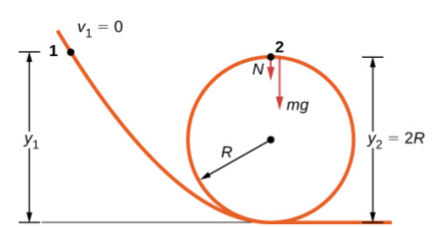
\includegraphics[width=\textwidth]{figures/loop.png}
\end{figure}
\end{column}
\end{columns}
\end{frame}

\section{Lab Activity: Gravitational Potential Energy and Work-Energy Theorem}

\begin{frame}{Lab Activity - See Lab Handout}
(See laboratory activity handout).
\end{frame}

\section{Lab Activity: Roller Coaster}

\begin{frame}{Lab Activity for Gravitational Potential Energy }
\small
\begin{columns}[T]
\begin{column}{0.33\textwidth}
\textbf{Materials (5 min)}:
\begin{itemize}
\item Pipe liner
\item A ball bearing
\item Scissors
\item Tape
\item Ruler
\end{itemize}
\end{column}
\begin{column}{0.33\textwidth}
\textbf{Build (10 min)}:
\begin{itemize}
\item Cut pipe liner in half, lengthwise
\item Shape the pipe liner into the shape on prior slide
\item Use tape to fix in place
\end{itemize}
\end{column}
\begin{column}{0.33\textwidth}
\textbf{Measure (15 minutes)}:
\begin{itemize}
\item Measure the initial height required to traverse loop
\item Compare to loop radius
\item Report the radius and ten initial height measurements
\end{itemize}
\end{column}
\end{columns}
\alert{\textbf{Bonus}: \textit{Two loops?}}
\end{frame}

\begin{frame}{Kinetic Energy and the Work-Energy Theorem}
\textit{Interactive simulation}:
\url{https://openstaxcollege.org/l/21PhETSimRamp}
\begin{itemize}
\item Push an object up the ramp (which includes friction)
\item Copy the energy plot to your lab notebook, and explain each feature of it.
\begin{enumerate}
\item Where is the energy constant?
\item Where is the energy changing?
\end{enumerate}
\end{itemize}
\end{frame}

\section{Power}

\begin{frame}{Power}
\textbf{Power} is the derivative of \textbf{work}:
\begin{align}
P =& \frac{dW}{dt} \\
W =& \int P dt
\end{align}
The unit of power is the Watt, or 1 J/s = 1 N m/s.
\end{frame}

\begin{frame}{Power}
A common scale for home power usage is the kW hr, or kilowatt hours, which is a unit of energy.  If a home consumes 1000 kW hr in one month, what is the average power consumed at a given time in this home?  (Hint: divide by the time of one month).
\begin{itemize}
\item A: 0.1 kW
\item B: 1.4 kW
\item C: 10 kW
\item D: 1.2 MW
\end{itemize}
\textit{According to Google, central AC uses about 3500 W for a home.  Think about this the next time you get your electric bill...}
\end{frame}

\begin{frame}{Power}
Since $P = \frac{dW}{dt}$ we may show that $P = \vec{F} \cdot \vec{v}$.  (Example).
\end{frame}

\section{Definition of Conservative Force}

\begin{frame}{Definition of Conservative Force}
\begin{tcolorbox}[colback=white,colframe=red!40!blue,title=Definition of Conservative Force]
\alert{Let $\vec{F}(x,y)$ describe some \textit{force field}.  The field is \textbf{conservative} if the line integral around a closed path is zero: \\
\begin{equation}
\oint_{p} \vec{F} \cdot d\vec{r} = 0
\end{equation}
Returning the system to the same point implies no net work.}
\end{tcolorbox}
\begin{tcolorbox}[colback=white,colframe=red!40!blue,title=Corollary 1]
\begin{equation}
\frac{dF_y}{dx} = \frac{dF_x}{dy}
\end{equation}
\end{tcolorbox}
\end{frame}

\begin{frame}{Definition of Conservative Force}
Consider the case of gravity: $\vec{F}(x,y) = 0\hat{i} -mg \hat{j}$.  So it depends neither on $x$ nor $y$.  Let's check that it is conservative:
\begin{align}
\frac{dF_y}{dx} =& 0 \\
\frac{dF_x}{dy} =& 0 \\
\frac{dF_y}{dx} =& \frac{dF_x}{dy}
\end{align}
\end{frame}

\begin{frame}{Definition of Conservative Force}
Which force is conservative?
\begin{itemize}
\item A: $\vec{F} = x^2\hat{i}+y^2\hat{j}$
\item B: $\vec{F} = x\hat{i}-y^2\hat{j}$
\item C: $\vec{F} = -\hat{i}+y\hat{j}$
\item D: $\vec{F} = x^2\hat{i}-y\hat{j}$
\end{itemize}
\textit{Hint: when you picture a conservative force, picture symmetry}.
\end{frame}

\section{Conclusion}

\begin{frame}{Unit 6 Summary}
\begin{enumerate}
\item \alert{Work} has a scientifically precise definition
\begin{itemize}
\item Units
\item As a product of force and displacement vectors
\end{itemize}
\item Kinetic Energy and the \alert{Work-Energy Theorem}
\item Gravitational potential energy
\begin{itemize}
\item Potential energy
\item \textit{Simplifying otherwise complex calculations}
\item Potential energy near Earth's surface
\item ...in space
\end{itemize}
\item Definition of a \textbf{conservative force}
\begin{itemize}
\item Relationship between conservative forces and potential energy
\item Conservation of energy for conservative forces
\end{itemize}
\end{enumerate}
\end{frame}

\end{document}
